\section{Dataset and Exploratory Analysis}
\label{sec:dataset}
\subsection{Dataset and partitioning}
Fashion-MNIST contains 60,000 official training images and 10,000 official test
images \cite{fresh_fashion,dataset_repository}. Each image has $28\times28$
grayscale pixels, with integer intensities from 0 to 255. There are ten labels,
listed in Table~\ref{tab:labels}.

\begin{table}[H]\centering
\caption{Fashion-MNIST labels used throughout the report.}\label{tab:labels}
\begin{tabular}{clcl}\toprule
Label & Category & Label & Category\\\midrule
0 & T-shirt/top & 5 & Sandal\\
1 & Trouser & 6 & Shirt\\
2 & Pullover & 7 & Sneaker\\
3 & Dress & 8 & Bag\\
4 & Coat & 9 & Ankle boot\\\bottomrule
\end{tabular}
\end{table}

The official training source is divided into training and validation partitions
with a stratified 90/10 split and seed 42. The official test partition is kept
separate. Every class has the same number of examples within each partition.

\begin{table}[H]\centering
\caption{Fixed partitions and their roles.}\label{tab:splits}
\begin{tabularx}{\linewidth}{lrrX}\toprule
Partition & Images & Per class & Purpose\\\midrule
Training & 54,000 & 5,400 & Fit normalization and update weights.\\
Validation & 6,000 & 600 & Select the checkpoint by validation loss.\\
Test & 10,000 & 1,000 & Evaluate the selected checkpoint.\\\bottomrule
\end{tabularx}
\end{table}

The cached training and validation indices are disjoint and together cover the
60,000 training-source images. The saved dataset audit found no exact duplicate
images within the partitions or across their boundaries. The audit compares raw
image hashes, so it does not rule out near duplicates or related products.
No images are removed or reassigned.

\subsection{Exploratory analysis}
\subsubsection{Class balance and visual variation}
Each class represents 10\% of every partition. The training procedure therefore
uses the same loss weight for every class. Equal class counts still allow large
differences in difficulty, which motivates the per-class analysis in Section~5.

Figure~\ref{fig:training_examples} shows three training examples per class,
selected with seed 42. Trousers, bags and footwear have relatively distinctive
overall shapes. Upper-body garments share a torso and sleeves, while their
outlines and brightness vary within each class. These examples illustrate the
task; three images cannot establish how often a particular pattern occurs.

Descriptive statistics and visual summaries use the 54,000 training images.
Validation and test images contribute only to structural checks and the
duplicate audit at this stage. This keeps held-out data separate from the
statistics used to prepare model inputs.

\clearpage
\begin{figure}[H]\centering
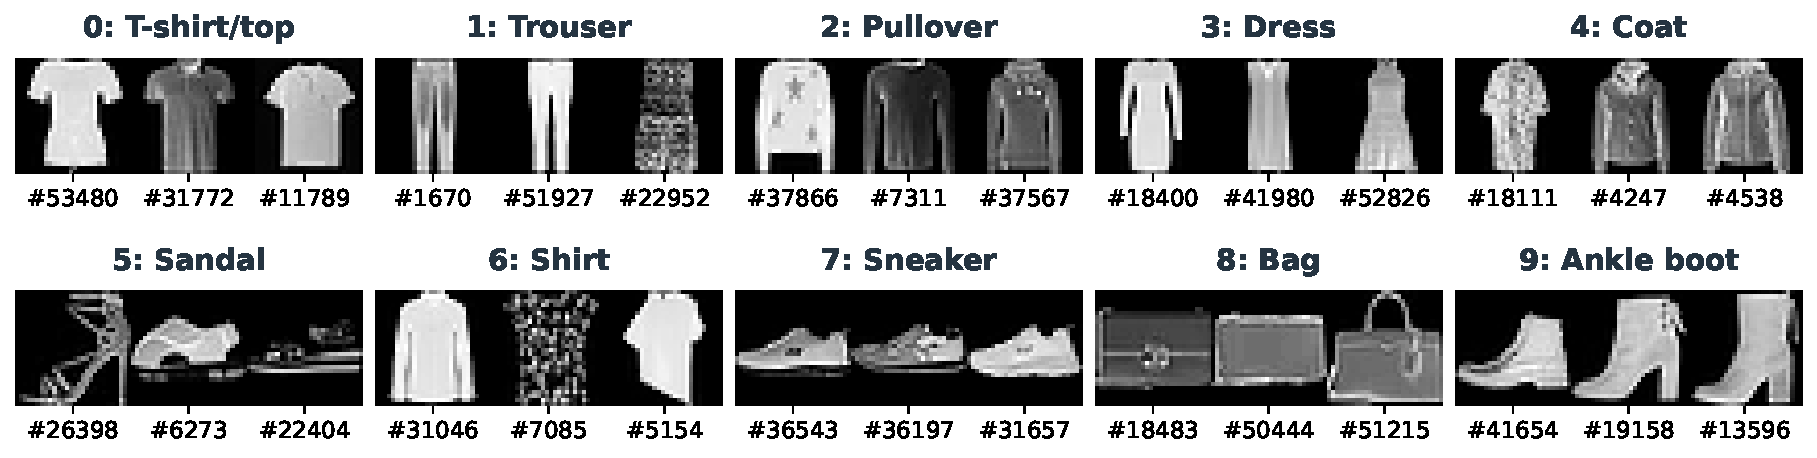
\includegraphics[width=.97\linewidth]{02_training_examples.pdf}
\caption{Three training examples per class. Numbers identify the original
training-source indices. All images use the same 0--255 display range.}
\label{fig:training_examples}
\end{figure}

\subsubsection{Pixel intensity and background}
The training subset contains 42,336,000 pixels. Their raw mean is 72.9833 and
their population standard deviation is 90.0557. Approximately 50.21\% of these
pixels are exactly zero, but none of the training images is entirely blank.
A large background region therefore does not indicate an empty sample.

\begin{figure}[H]\centering
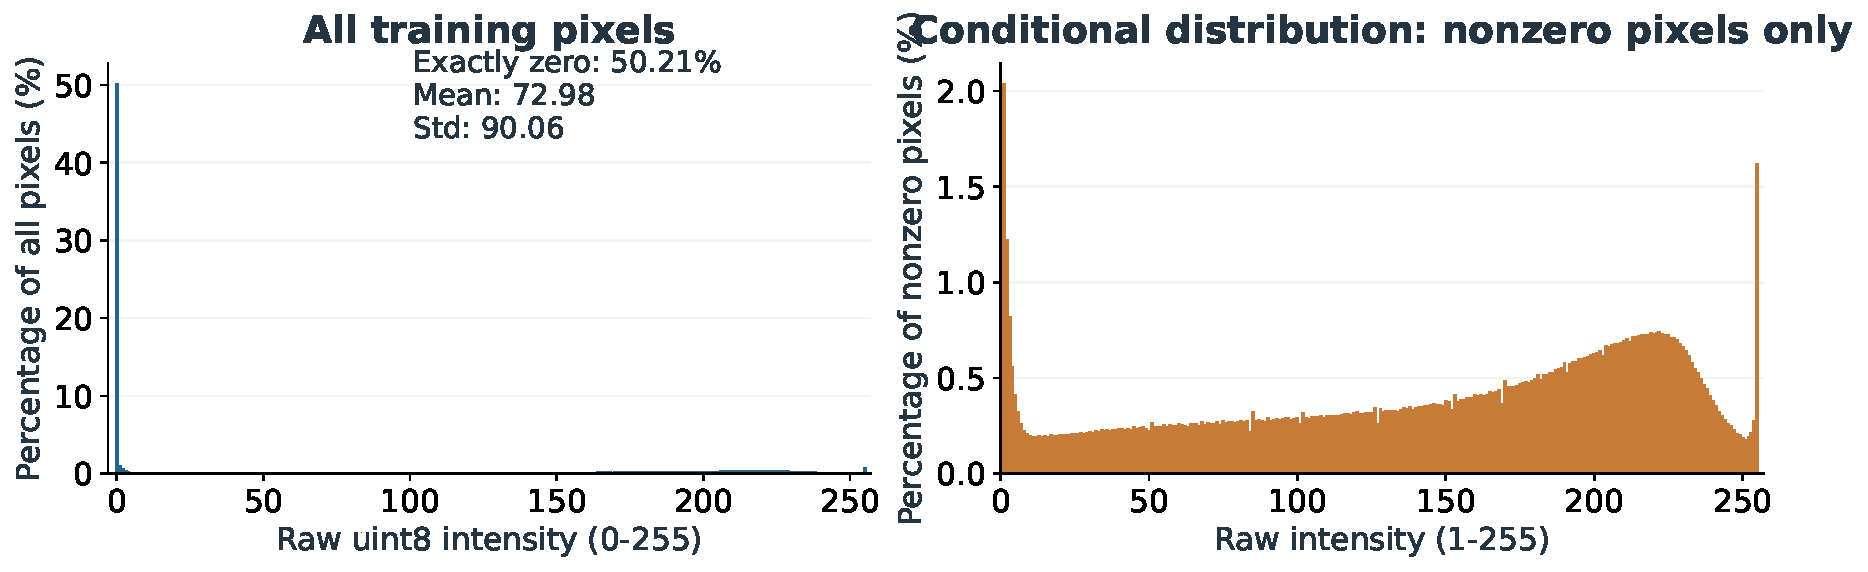
\includegraphics[width=.96\linewidth]{03_pixel_distribution.pdf}
\caption{Training-pixel intensity distributions. The left panel includes all
pixels; the right panel conditions on positive intensities. The panels use
different denominators.}\label{fig:pixels}
\end{figure}

The large zero-intensity mass is consistent with the dark background visible
in the samples. Positive pixels include both object interiors and faint edges.
Counting nonzero pixels is useful for describing coverage, but is not a semantic
segmentation of the clothing item.

\clearpage
\subsubsection{Brightness, coverage and spatial structure}
For each image, mean brightness is the average of its 784 raw intensities.
Nonzero coverage is the fraction of pixels with intensity greater than zero.
Table~\ref{tab:brightness} summarizes these quantities by class.

\begin{table}[H]\centering
\caption{Training statistics by class. Each row represents 5,400 images.
Brightness SD is the standard deviation of image means.}
\label{tab:brightness}
\begin{tabular}{lrrr}\toprule
Class & Mean brightness & Brightness SD & Nonzero coverage (\%)\\\midrule
\tabledata{generated/eda_rows.tex}
\bottomrule\end{tabular}
\end{table}

Sandal has the lowest mean brightness, 34.87, while Coat has the highest,
98.15. Pullover has the largest mean nonzero coverage, 64.84\%. These are
class averages, not decision rules: individual images vary and the class
distributions overlap.

\begin{figure}[H]\centering
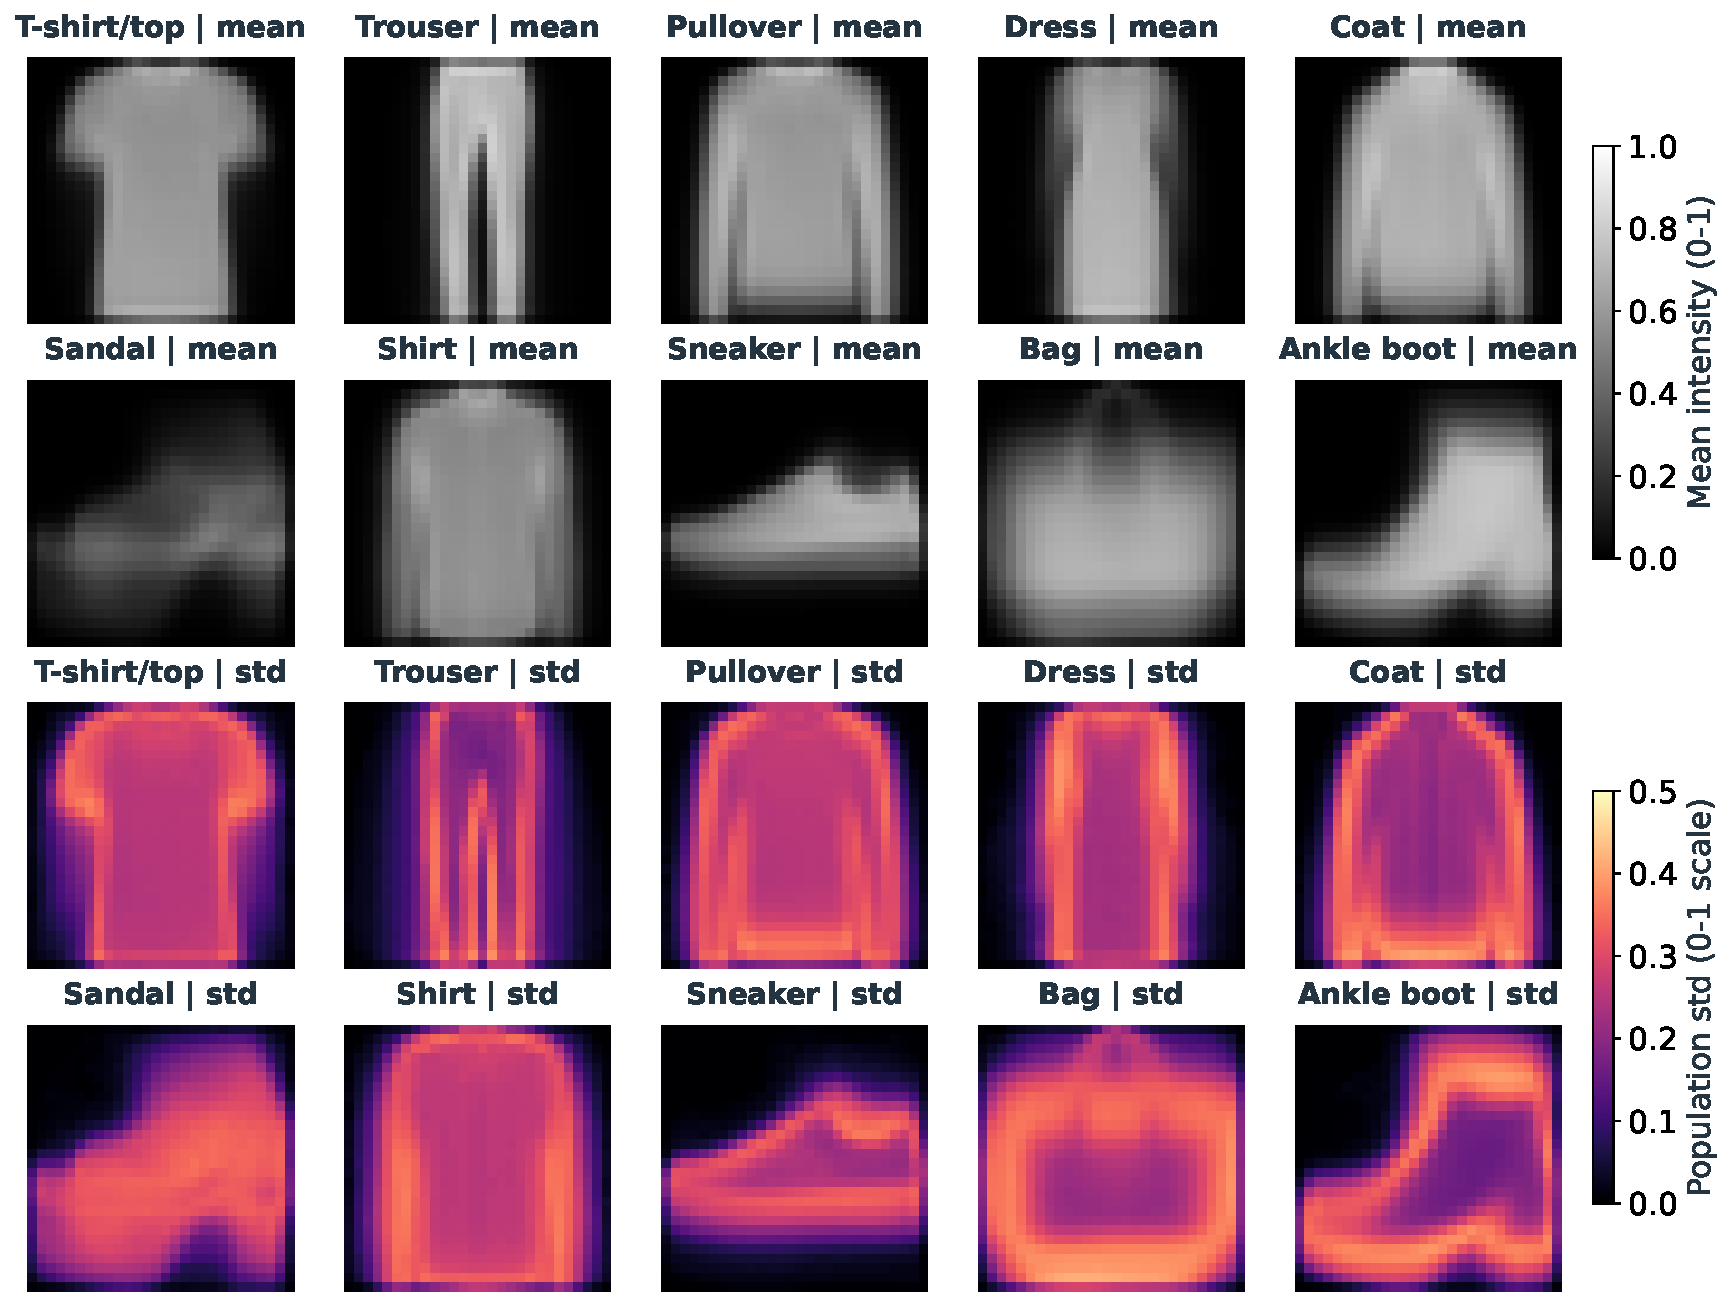
\includegraphics[width=.76\linewidth]{05_spatial_statistics.pdf}
\caption{Training class-average images and pixelwise standard deviations.
The average highlights recurring silhouettes; the standard deviation shows
where images within a class differ.}\label{fig:spatial}
\end{figure}

The class averages preserve broad silhouettes while removing much individual
detail. The recorded cosine similarity between the uncentered Coat and Shirt
averages is 0.9873, the highest pair in the audit. This suggests a useful question
for error analysis: do models confuse upper-body garments? It does not measure
the separability of individual images or prove a particular confusion rate.

\clearpage
\subsection{Preprocessing}
\label{sec:preprocessing}
\subsubsection{Scaling and training-only standardization}
Raw intensities are first converted to floating-point values and divided by 255.
The training mean $\mu$ and population standard deviation $\sigma$ are then
computed over all training pixels. For a raw pixel $X_{r,c}$, the normalized
value is
\[
Z_{r,c}=\frac{X_{r,c}/255-\mu}{\sigma},
\qquad \mu=0.286209,\quad \sigma=0.353160.
\]
The values shown are rounded; the code uses the full-precision cached constants.
Validation and test images reuse these constants without fitting their own
statistics. This prevents held-out images from influencing normalization.

The transformation preserves resolution and pixel ordering. Raw values 0 and
255 map to approximately $-0.810$ and $2.021$, without clipping.

\subsubsection{Input arrangements}
The same standardized image is rearranged to match each model:
Linear and MLP receive 784 pixels in row-major order; CNN receives a single
channel image grid; LSTM receives 28 top-to-bottom rows; and Transformer
receives 49 non-overlapping $4\times4$ patches in raster order.

\begin{figure}[H]\centering
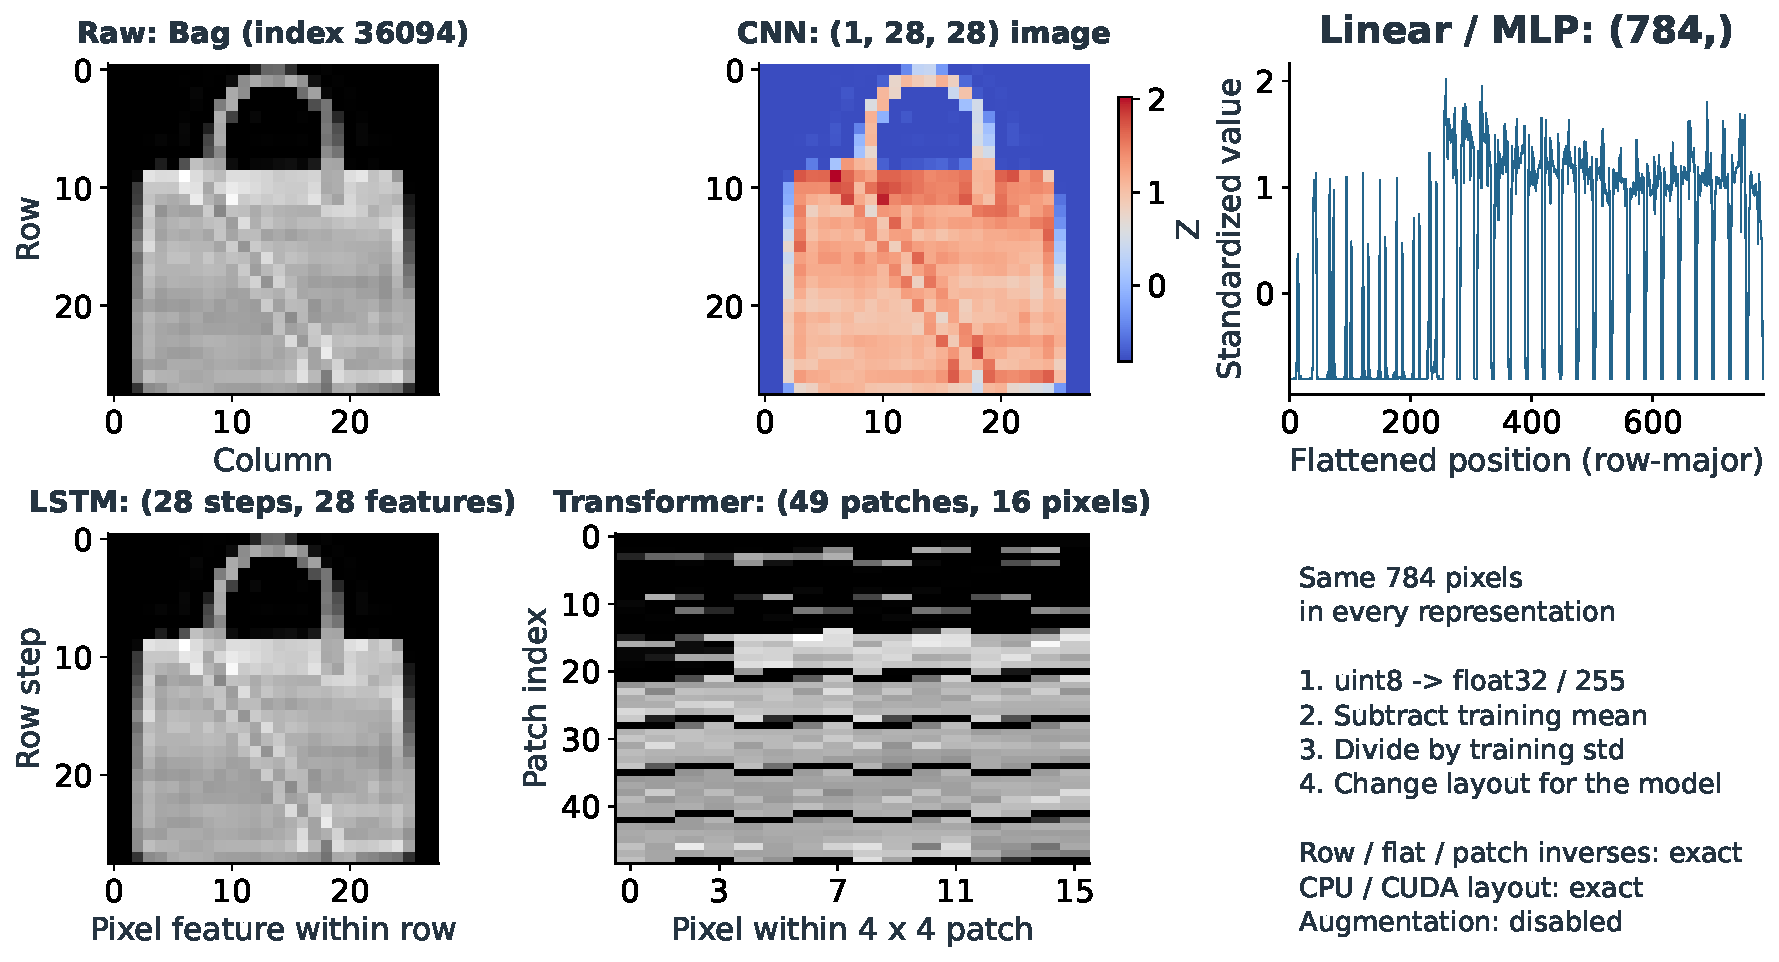
\includegraphics[width=.82\linewidth]{07_preprocessing_representations.pdf}
\caption{Equivalent input arrangements for the same image. Each arrangement
retains all 784 standardized pixel values. Learned embeddings belong to the
model, after preprocessing.}\label{fig:representations}
\end{figure}

For Transformer patch coordinates $a,b\in\{0,\ldots,6\}$ and local coordinates
$u,v\in\{0,\ldots,3\}$, the mapping is
\[
P_{7a+b,\,4u+v}=Z_{4a+u,\,4b+v}.
\]
Thus $49\times16=784$ values are retained without padding or interpolation.
For the LSTM, the sequence describes ordered positions in one static image;
it is not a time series of different images.

\subsubsection{Augmentation and verification}
No rotations, flips, resizing, denoising or other augmentation are applied.
The recorded preprocessing checks confirm that the standardized training data
has mean approximately zero and population standard deviation approximately
one, with deviations below $10^{-6}$. They also confirm pixel ordering, exact
patch reconstruction and CPU/CUDA agreement.

The following methodology compares ways of using this shared image information,
with particular interest in local structure and similar garment silhouettes.
